\newpage
\section{Diagramas de secuencia}
A continuación se describe la interacción de nuestras entidades de negocio y el ciclo de vida que tendrán en la aplicación. También se detalla la interacción,mensajes y la lógica implementada por cada uno de los diferentes escenarios.\par
\subsection{Registro}
El registro de un usuario nuevo consiste en capturar el correo, nombre y una contraseña. Esta captura sera tratada como un JSON el cual viajara atravéz de un método POST. Gateway se encargara de redirigir esta petición al servicio de registro. Este servicio viajara hacia RDS donde se enviara un INSERT para registrar los datos. Si el usuario y la contraseña se encuentra repetido, se enviara un mensaje de error, como se muestra en la figura 3.7
\begin{figure}[h!]
	\centering
	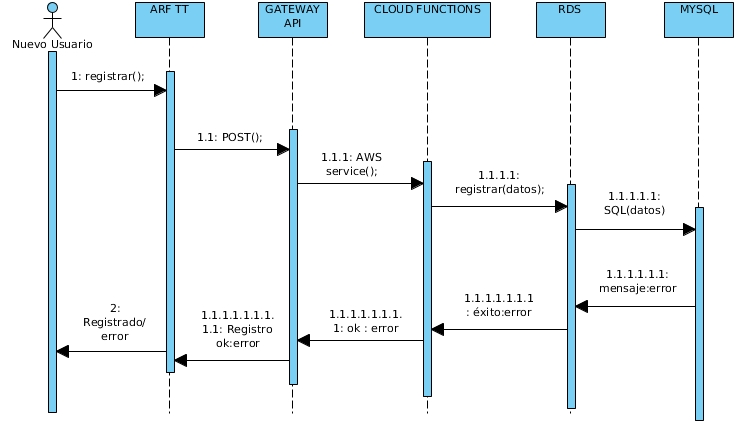
\includegraphics[width=14cm,height=8cm]{imagenes/analisis/DSregistrarUsuario.jpg}
	\caption{Diagrama de secuencia - Registrar usuario.}
	\label{fig:analogo}
\end{figure} 
\subsection{Login}
La validación de credenciales comienza con capturar el correo y contraseña  de un usuario registrado. Esta información sera tratada como un objeto JSON, el cual se mandara por una método POST. La API Gateway direccionara la petición a un Servicio AWS y  comparara la información en la instancia creada en RDS de un motor de base de datos MySQL. RDS se encargara de generar la conexión y consulta a la base de datos. La petición regresara con un mensaje si hubo coincidencia, de lo contrario se enviara un error a la interfaz de usuario.
\begin{figure}[h!]
	\centering
	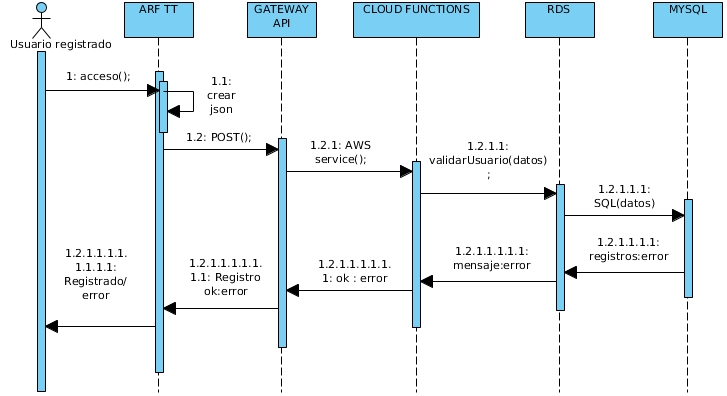
\includegraphics[width=14cm,height=8cm]{imagenes/analisis/DSacceso.jpg}
	\caption{Diagrama de secuencia - Registrar Acceso.}
	\label{fig:analogo}
\end{figure} 
\subsection{Recuperar contraseña}\par
La recuperación de credenciales inicia con la función recuperar, en ella se captura el correo de un usuario y posteriormente lo procesa a un objeto JSON. Esta información se mandara en un método POST. La API Gateway envía la petición a un Servicio AWS y en la instancia creada en RDS procesa un script que comparara el correo con la  información de MySQL, buscando alguna coincidencia. Si existe una coincidencia exacta, MySQL enviará el registro en un mensaje con la contraseña. Si no existe coincidencia se manda un mensaje de error. RDS se encargara de generar la conexión y consulta con el servicio de Amazon Web Services y nuestra instancia de MySQL en RDS.
\begin{figure}[h!]
	\centering
	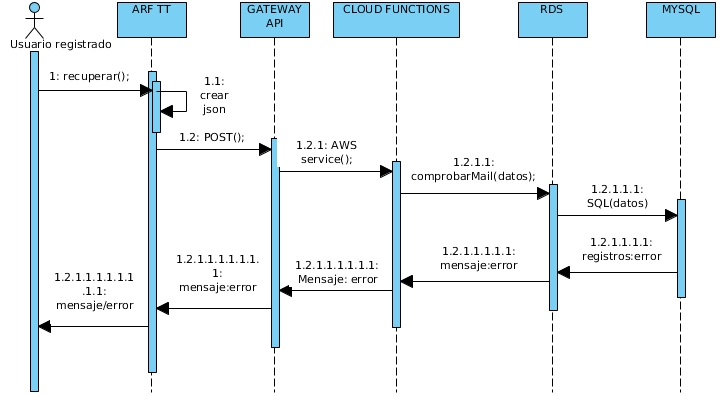
\includegraphics[width=14cm,height=8cm]{imagenes/analisis/DSrecuperarContra.jpg}
	\caption{Diagrama de secuencia - Recuperar contraseña.}
	\label{fig:analogo}
\end{figure} 
\newpage


